% \begin{figure}[htbp]
%     \vspace{-1.5cm}
%     \centering
%     % 子图 (a)
%     \begin{subfigure}[b]{0.495\textwidth}
%         \centering
%         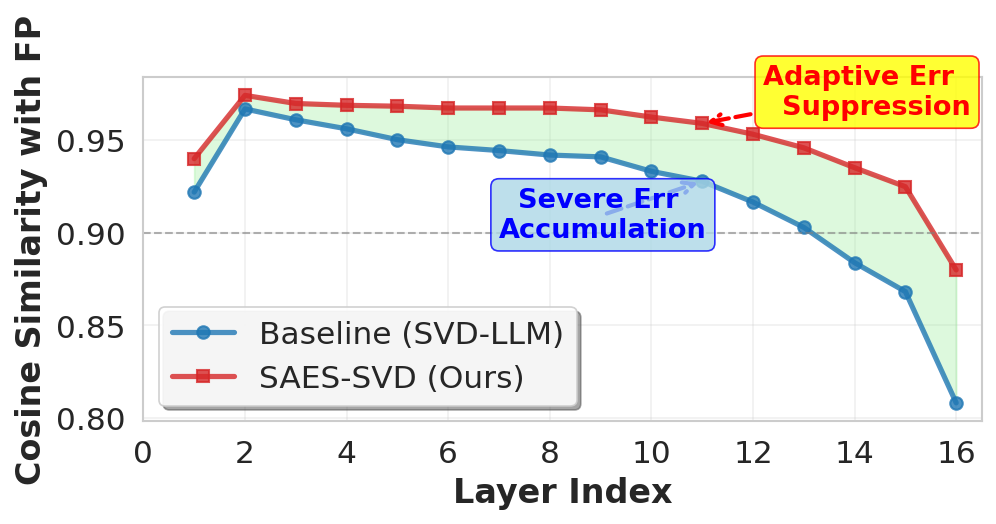
\includegraphics[width=\textwidth]{figs/error_accumulation_comparison.png}
%         \vspace{-5mm}
%         \caption{}
%         \label{fig:sub1}
%     \end{subfigure}
%     \hfill
%     % 子图 (b)
%     \begin{subfigure}[b]{0.495\textwidth}
%         \centering
%         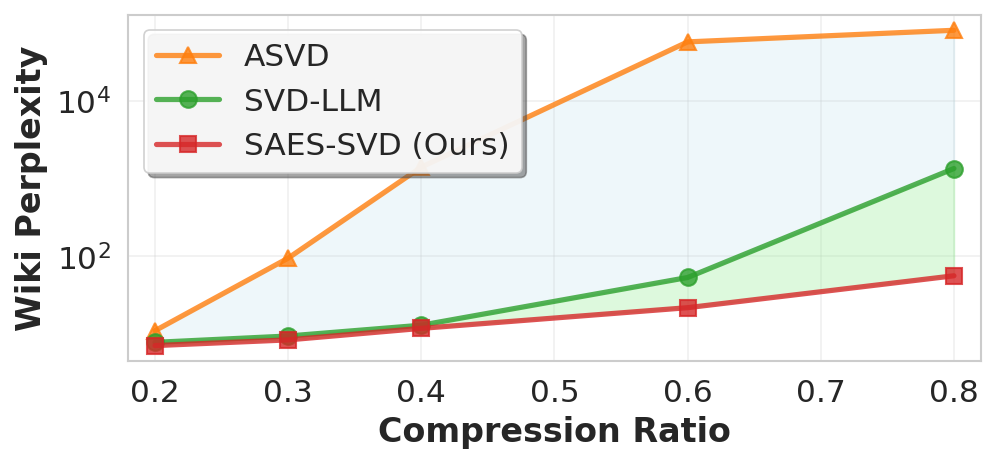
\includegraphics[width=\textwidth]{figs/perplexity_compression_comparison.png}
%         \vspace{-5mm}
%         \caption{}
%         \label{fig:sub2}
%     \end{subfigure}
%     \vspace{-0.6cm}
%     \caption{Comparison of SAES-SVD with baseline methods. 
%     \textbf{(a)} Cumulative error analysis on LLaMA-3.2-1B, showing the cosine similarity of compressed outputs with the original reference across layers. SAES-SVD effectively mitigates error accumulation by adaptively suppressing upstream deviations. 
%     \textbf{(b)} Perplexity on WikiText2 under varying compression ratios. SAES-SVD consistently achieves lower perplexity than ASVD and SVD-LLM.
%     % demonstrating robustness under high compression settings.
%     }
%     \label{fig intro}
%     \vspace{-0.2cm}
% \end{figure}


\begin{figure}[htbp]
    \vspace{-1.5cm}
    \centering

    % 子图 (a)
    \begin{subfigure}[b]{0.497\textwidth}
        \centering
        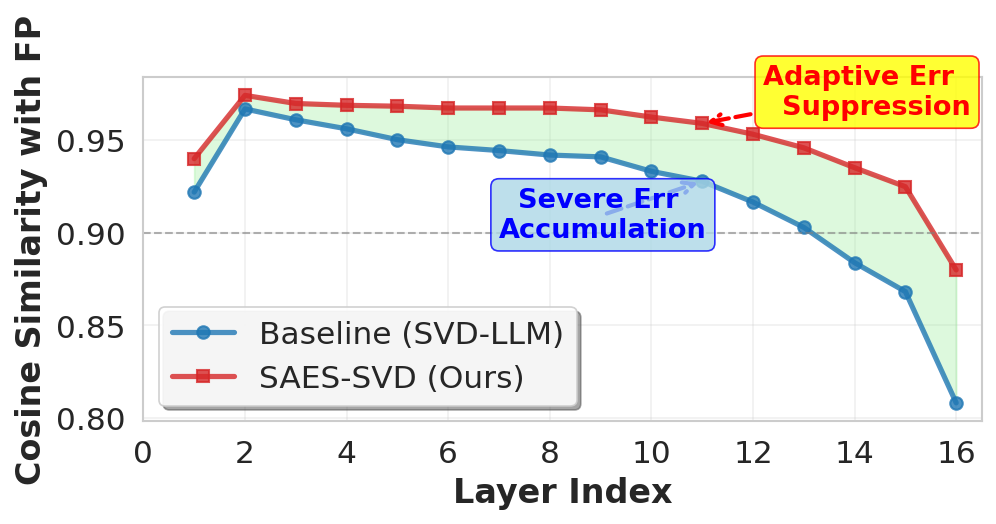
\includegraphics[width=\textwidth]{figs/error_accumulation_comparison.png}
        \vspace{-5mm}
        \caption{}
        \label{fig:sub1}
    \end{subfigure}
    \hfill
    % 子图 (b)
    \begin{subfigure}[b]{0.497\textwidth}
        \centering
        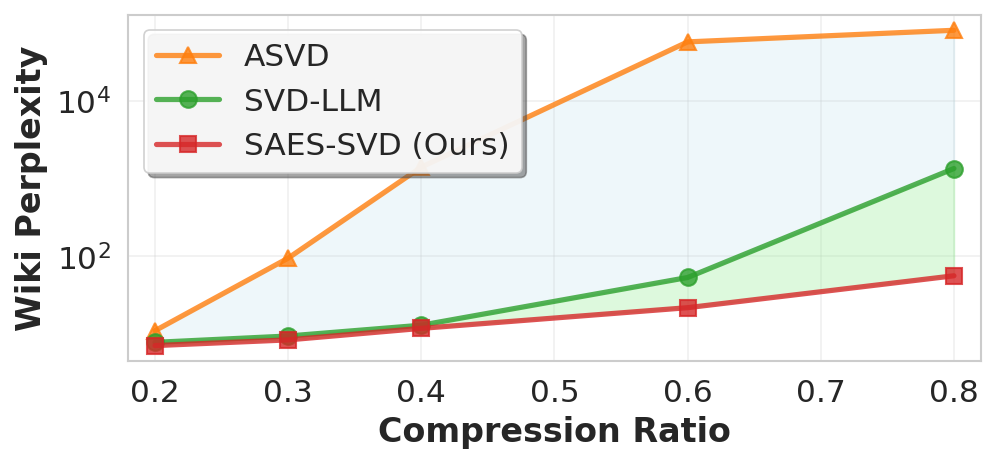
\includegraphics[width=\textwidth]{figs/perplexity_compression_comparison.png}
        \vspace{-5mm}
        \caption{}
        \label{fig:sub2}
    \end{subfigure}

    % 换行
    \vspace{-0.1cm}

    % 子图 (c)
    \begin{subfigure}[b]{0.496\textwidth}
        \centering
        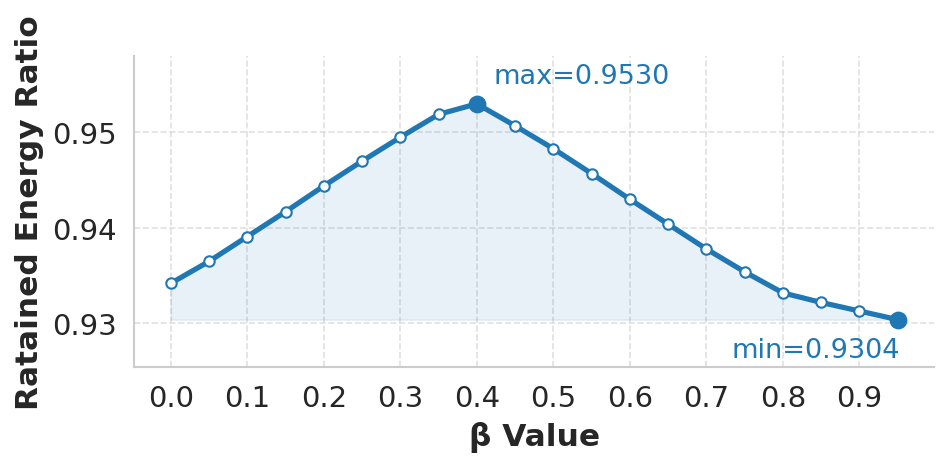
\includegraphics[width=\textwidth]{figs/ratio_of_differnet_beta.png}
        \vspace{-5mm}
        \caption{}
        \label{fig:sub3}
    \end{subfigure}
    \hfill
    % 子图 (d)
    \begin{subfigure}[b]{0.496\textwidth}
        \centering
        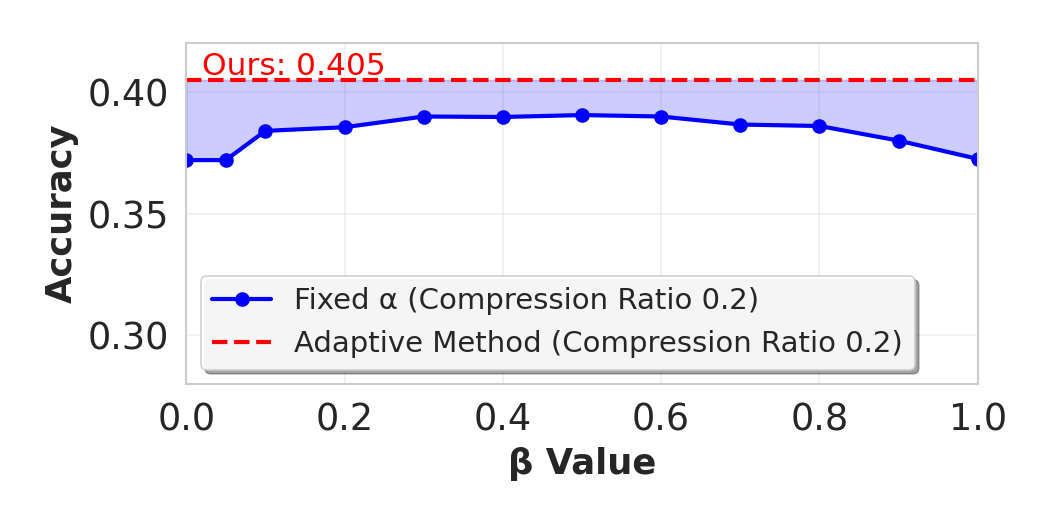
\includegraphics[width=\textwidth]{figs/3_plot_different_alpha.png}
        \vspace{-5mm}
        \caption{}
        \label{fig:sub4}
        \label{fig different alpha}
    \end{subfigure}
    \vspace{-0.6cm}
    \caption{
    \textbf{(a)} Cumulative error analysis on LLaMA-3-8B, showing the cosine similarity of compressed outputs with the original reference across layers. SAES-SVD effectively mitigates error accumulation by adaptively suppressing upstream deviations. 
    \textbf{(b)} Perplexity on WikiText2 under varying compression ratios. SAES-SVD consistently achieves lower perplexity than ASVD and SVD-LLM.
    \textbf{(c)} Retained Energy Ratio achieved by using different weighting coefficients for the cumulative error compensation term in with rank=128 compression for k-proj in the 14th Layer of LLaMA-3-8B. Here, for the sake of convenience, we use $\beta=\alpha/(1+\alpha)$ as the horizontal axis.
    \textbf{(d)} Effect of fixed versus adaptive weighting coefficients for the cumulative error compensation on average accuracy across 7 zero-shot benchmarks.
    }
    \label{fig:intro}
    \label{fig intro}
    \vspace{-0.2cm}
\end{figure}
